\ylDisplay{Vooluring} % Ülesande nimi
{Valter Kiisk} % Autor
{piirkonnavoor} % Voor
{2005} % Aasta
{G 4} % Ülesande nr.
{4} % Raskustase
{
% Teema: Elektriahelad
\ifStatement
Takisti takistuse määramiseks koostati kaks erinevat vooluringi kasutades voltmeetrit, ampermeetrit ja vooluallikat (vt joonist). Leidke avaldis takistuse $R$ arvutamiseks, kui vasakpoolse skeemi järgi mõõtes saadi voltmeetri näiduks $U_1$ ja ampermeetri näiduks $I_1$ ning parempoolse skeemi järgi mõõtes aga vastavalt $U_2$ ja $I_2$. Vooluallika elektromotoorjõud on muutumatu ning sisetakistus tühine. Mõõteriistade sisetakistused ei ole teada.

\begin{figure}[h]
	\centering
	\begin{minipage}[b]{0.25\textwidth}
		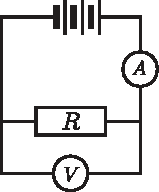
\includegraphics[width=\linewidth]{2005-v2g-04-yl1}
	\end{minipage}
	\hspace{30pt}
	\begin{minipage}[b]{0.3\textwidth}
		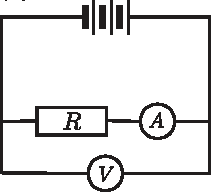
\includegraphics[width=\linewidth]{2005-v2g-04-yl2}
    \end{minipage}
\end{figure}

\fi


\ifHint
Ülesandes on neli tundmatut: vooluallika pinge, takisti takistus ning ampermeetri ja voltmeetri sisetakistused. Nelja tundmatu jaoks on vaja nelja võrrandit ning need tulenevad ülesandes antud ampermeetri ja voltmeetri näitudest.
\fi


\ifSolution
Teisest skeemist näeme, et vooluallika elektromotoorjõud $\mathcal E$ võrdub voltmeetri näiduga,
\[
\mathcal E = U_2.
\]
Seega esimese skeemi jaoks
\[
U_1 + I_1r_a = \mathcal E = U_2,
\]
teise skeemi jaoks
\[
I_2R + I_2r_a = U_2,
\]
kus $r_a$ on ampermeetri sisetakistus. Viimase elimineerimisel saame
\[
R=\frac{I_{1} U_{2}+I_{2} U_{1}-I_{2} U_{2}}{I_{1} I_{2}}=\frac{U_{2}}{I_{2}}+\frac{U_{1}}{I_{1}}-\frac{U_{2}}{I_{1}}.
\]
\fi
}